\documentclass[aspectratio=169,11pt]{beamer}
\usepackage[T1]{fontenc}
\usepackage{lmodern}
\usepackage{amsmath,amssymb,booktabs,listings}
\usetheme{Madrid}
\usecolortheme{dolphin}
\setbeamertemplate{blocks}[rounded][shadow=false]
\definecolor{Navy}{HTML}{15345C}
\definecolor{Teal}{HTML}{2266B3}
\definecolor{Coral}{HTML}{D6603C}
\definecolor{Mist}{HTML}{EFF5FC}
\setbeamercolor{normal text}{fg=Navy,bg=white}
\setbeamercolor{structure}{fg=Teal}
\setbeamercolor{frametitle}{fg=white,bg=Navy}
\setbeamercolor{title}{fg=white,bg=Navy}
\setbeamercolor{subtitle}{fg=white}
\setbeamercolor{alerted text}{fg=Teal}
\setbeamercolor{palette primary}{fg=white,bg=Teal}
\setbeamercolor{palette secondary}{fg=white,bg=Navy}
\setbeamercolor{palette tertiary}{fg=white,bg=Navy}
\setbeamercolor{block title}{fg=white,bg=Teal}
\setbeamercolor{block body}{fg=Navy,bg=Mist}
\setbeamerfont{title}{size=\Huge,series=\bfseries}
\setbeamerfont{frametitle}{size=\Large,series=\bfseries}
\setbeamertemplate{navigation symbols}{}
\setbeamertemplate{itemize items}[circle]
\setbeamersize{text margin left=9mm,text margin right=9mm}
\setbeamertemplate{headline}{}
\setbeamertemplate{footline}{%
 \leavevmode\hbox{%
 \begin{beamercolorbox}[wd=.84\paperwidth,ht=2.8ex,dp=1.2ex,leftskip=9mm]{palette secondary}%
 \scriptsize DRP\enspace\textbar\enspace DDPM Learning
 \end{beamercolorbox}%
 \begin{beamercolorbox}[wd=.16\paperwidth,ht=2.8ex,dp=1.2ex,center]{palette primary}%
 \scriptsize\insertframenumber\,/\,\inserttotalframenumber
 \end{beamercolorbox}}}
\lstset{language=Python,basicstyle=\ttfamily\small,keywordstyle=\color{Teal}\bfseries,
 stringstyle=\color{Coral},showstringspaces=false,columns=fullflexible,keepspaces=true,
 frame=none,backgroundcolor=\color{Mist},xleftmargin=2mm,xrightmargin=2mm,
 aboveskip=3mm,belowskip=3mm,breaklines=false}
\newcommand{\ddpmref}{\vfill{\tiny\color{gray}Ho, Jain, and Abbeel (2020), \href{https://arxiv.org/abs/2006.11239}{Denoising Diffusion Probabilistic Models}.}}
\title{Denoising diffusion\\probabilistic models}
\subtitle{DDPM on the same four-component Gaussian mixture}
\author{\texorpdfstring{Directed Reading Program\\Florida State University}{Directed Reading Program, Florida State University}}
\date{}
\begin{document}

\begin{frame}
\titlepage
\vspace{-5mm}
\centering\textcolor{Teal}{Forward noise \quad Noise prediction \quad Reverse sampling}
\end{frame}

\begin{frame}{The same generation problem}
\large
\[p_{\mathrm{data}}(x)=\frac14\sum_{j=1}^4\mathcal N(x;\mu_j,0.35^2I_2)\]
\normalsize
\[\mu_1=(-2,-2),\quad\mu_2=(-2,2),\quad
\mu_3=(2,-2),\quad\mu_4=(2,2)\]
\vspace{4mm}
\begin{itemize}\setlength\itemsep{4mm}
\item Start sampling from a two-dimensional standard Gaussian.
\item Produce new points near all four centers with the right spread.
\item Use fresh real samples to check the generated distribution.
\end{itemize}
\end{frame}

\begin{frame}{What changes from the ODE lesson?}
\begin{center}\small
\begin{tabular}{p{.23\textwidth}p{.29\textwidth}p{.32\textwidth}}
\toprule
& Flow matching & DDPM here\\\midrule
Network predicts & Velocity & Added noise\\[3mm]
Training states & Straight interpolations & Gaussian-corrupted data\\[3mm]
Sampling & ODE Euler steps & Gaussian reverse transitions\\[3mm]
Randomness & Initial point & Initial point and reverse steps\\[3mm]
Endpoints & Noise at 0, data at 1 & Data at 0, noise at $T$\\\bottomrule
\end{tabular}
\end{center}
\vspace{3mm}
We now implement a stochastic DDPM sampler, not an ODE flow.
\end{frame}

\begin{frame}[fragile]{1. Create the training data}
\begin{columns}[c]
\begin{column}{.55\textwidth}
\begin{lstlisting}[basicstyle=\ttfamily\footnotesize]
centers = torch.tensor([
    [-2., -2.], [-2., 2.],
    [2., -2.], [2., 2.]
])
sigma = 0.35

def sample_data(n):
    labels = torch.randint(4, (n,))
    return (centers[labels]
            + sigma * torch.randn(n, 2))

x_train = sample_data(4096)
\end{lstlisting}
\small Direct sampling is known here. Learning the distribution is a teaching exercise.
\end{column}
\begin{column}{.42\textwidth}
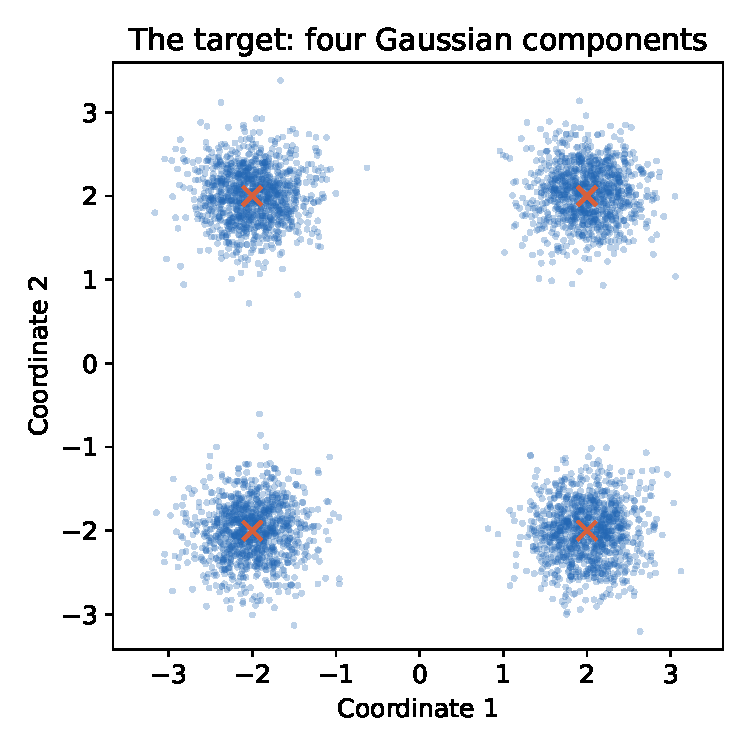
\includegraphics[width=\linewidth]{figures/training_data.pdf}
\end{column}
\end{columns}
\end{frame}

\begin{frame}{2. A forward step adds Gaussian noise}
\large
\[\boxed{x_t=\sqrt{1-\beta_t}\,x_{t-1}+\sqrt{\beta_t}\,\eta_t}\]
\[\eta_t\sim\mathcal N(0,I_2)\]
\normalsize
\begin{itemize}\setlength\itemsep{4mm}
\item Multiply the current point by a factor slightly below 1.
\item Add fresh Gaussian noise, independently at every step.
\item Repeat until the data distribution is nearly standard Gaussian.
\end{itemize}
\ddpmref
\end{frame}

\begin{frame}[fragile]{The noise schedule is fixed before training}
\begin{lstlisting}
T = 1000
beta = torch.linspace(0.0001, 0.02, T)
alpha = 1 - beta
alpha_bar = torch.cumprod(alpha, dim=0)
\end{lstlisting}
\vspace{3mm}
$\beta_t$ is the variance of the fresh noise in one forward step.\\[3mm]
$\alpha_t=1-\beta_t$ is the squared signal multiplier for that step.\\[3mm]
\alert{Indexing:} Python \texttt{k} means mathematical timestep $t=k+1$.\\[2mm]
\texttt{alpha\_bar[0]} therefore represents $\bar\alpha_1$, not $\bar\alpha_0$.
\end{frame}

\begin{frame}{Cumulative signal retention}
\large
\[\bar\alpha_t=\prod_{s=1}^{t}\alpha_s,\qquad\bar\alpha_0=1\]
\normalsize
\begin{center}
\begin{tabular}{ll}
\toprule
Quantity & Meaning\\\midrule
$\beta_t$ & Variance of newly added noise\\[3mm]
$\alpha_t$ & Signal retention in one step\\[3mm]
$\bar\alpha_t$ & Cumulative squared signal coefficient\\\bottomrule
\end{tabular}
\end{center}
\vspace{4mm}
The noise level is determined by the entire schedule up to $t$.
\end{frame}

\begin{frame}{A shortcut to any forward noise level}
\large
\[\boxed{x_t=\sqrt{\bar\alpha_t}\,x_0+\sqrt{1-\bar\alpha_t}\,\varepsilon}\]
\[\varepsilon\sim\mathcal N(0,I_2)\]
\normalsize
\begin{itemize}\setlength\itemsep{3mm}
\item This samples the exact conditional marginal $q(x_t\mid x_0)$.
\item $\varepsilon$ represents aggregate noise, not only the final step's noise.
\item Training can jump directly to a randomly selected timestep.
\end{itemize}
\vspace{3mm}
Separate shortcut draws at different times are not a Markov trajectory.
\ddpmref
\end{frame}

\begin{frame}{Forward diffusion dissolves the four clusters}
\begin{center}
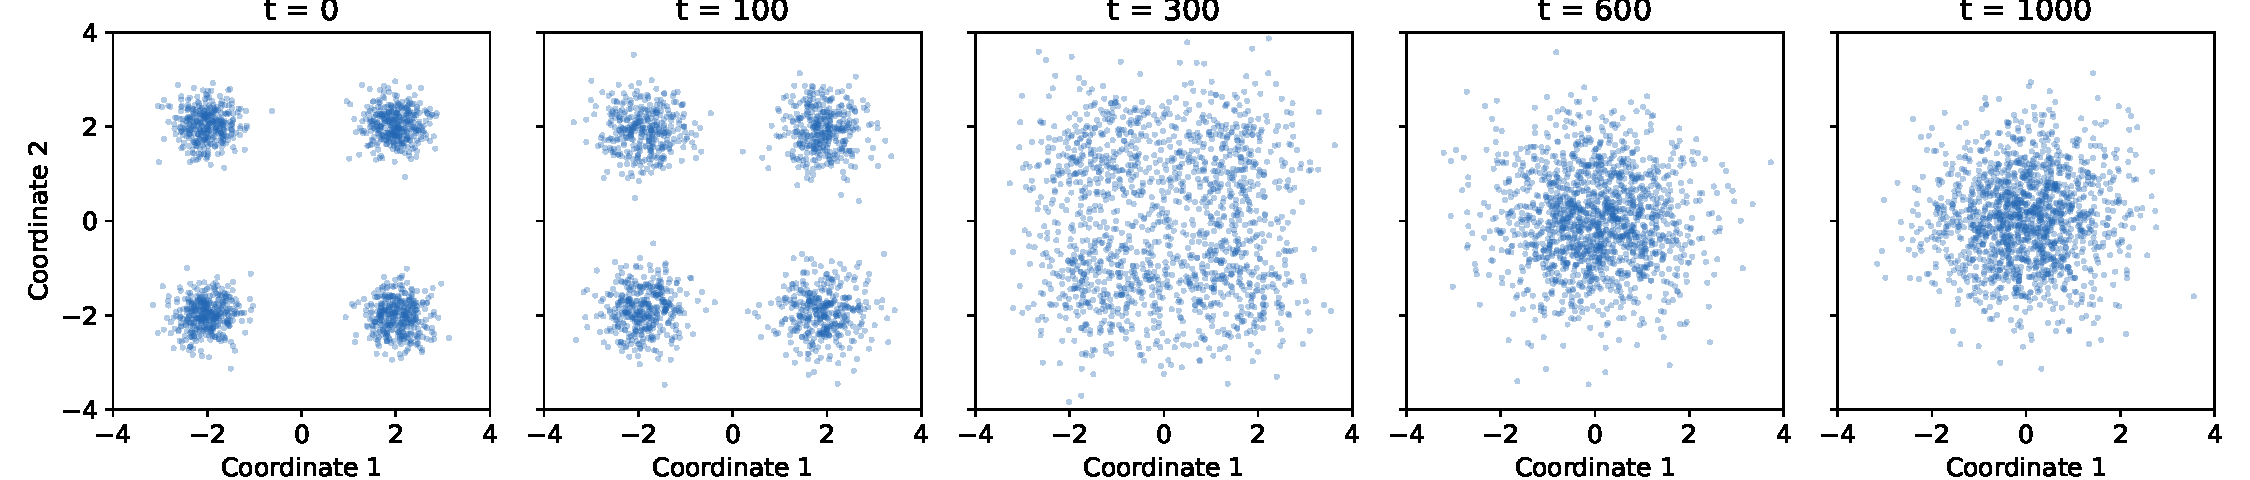
\includegraphics[width=\textwidth]{figures/forward_noising.pdf}
\end{center}
\vspace{4mm}
These panels follow one forward Markov simulation for the same 1,500 points.\\[3mm]
Each forward step uses independent noise. The forward process has no learned parameters.
\end{frame}

\begin{frame}{Why standard Gaussian noise is a reasonable start}
\large
\[\bar\alpha_T\approx0.00004036,\qquad\sqrt{\bar\alpha_T}\approx0.00635\]
\normalsize
\vspace{4mm}
The clean-data contribution is very small by $T=1000$.\\[4mm]
For this mixture, the four terminal component centers are near zero and their variances are near 1.\\[4mm]
The terminal distribution is close to standard Gaussian, not exactly equal.\\[4mm]
Shortening the schedule without checking residual signal can invalidate the initialization.
\end{frame}

\begin{frame}[fragile]{3. The network predicts noise}
\begin{columns}[c]
\begin{column}{.48\textwidth}
\begin{lstlisting}
model = nn.Sequential(
    nn.Linear(3, 64),
    nn.SiLU(),
    nn.Linear(64, 64),
    nn.SiLU(),
    nn.Linear(64, 2)
)
\end{lstlisting}
\end{column}
\begin{column}{.47\textwidth}
\[\text{Input: }(x_t^{(1)},x_t^{(2)},t/T)\]
\[\text{Output: }\varepsilon_\theta(x_t,t)\]
\small
Two noise coordinates, not a velocity.\\[4mm]
4,546 trainable parameters.\\[4mm]
Time in the equations is shorthand for the normalized network input.
\end{column}
\end{columns}
\end{frame}

\begin{frame}[fragile]{One training example at a random timestep}
\begin{lstlisting}[basicstyle=\ttfamily\footnotesize]
k = torch.randint(T, (256,))
noise = torch.randn_like(x0)
a = alpha_bar[k].reshape(-1, 1)
xt = a.sqrt() * x0 + (1 - a).sqrt() * noise
t = (k + 1).reshape(-1, 1) / T
prediction = model(torch.cat([xt, t], dim=1))
\end{lstlisting}
\vspace{4mm}
\texttt{xt}: $256\times2$, \texttt{t}: $256\times1$, input: $256\times3$.\\[3mm]
The target is \texttt{noise}, the same noise we used to construct \texttt{xt}.
\end{frame}

\begin{frame}[fragile]{4. Noise-prediction mean squared error}
\large
\[L=\frac{1}{2B}\sum_{i=1}^B
\left\|\varepsilon_i-\varepsilon_\theta(x_{t_i},t_i)\right\|^2\]
\normalsize
\begin{lstlisting}
loss_fn = nn.MSELoss()
optimizer = torch.optim.Adam(model.parameters(), lr=0.001)
\end{lstlisting}
\vspace{3mm}
PyTorch averages over the batch and both coordinates.\\[3mm]
We use uniformly sampled timesteps and the simplified DDPM objective, not the full variational likelihood bound.
\ddpmref
\end{frame}

\begin{frame}[fragile]{5. Training: construct noisy inputs}
\begin{lstlisting}[basicstyle=\ttfamily\footnotesize]
history = []
for step in range(10000):
    x0 = x_train[torch.randint(len(x_train), (256,))]
    k = torch.randint(T, (256,))
    noise = torch.randn_like(x0)
    a = alpha_bar[k].reshape(-1, 1)
    xt = a.sqrt() * x0 + (1 - a).sqrt() * noise
    t = (k + 1).reshape(-1, 1) / T
    prediction = model(torch.cat([xt, t], dim=1))
    loss = loss_fn(prediction, noise)
\end{lstlisting}
\vspace{3mm}
No full forward chain is needed for each training example.
\end{frame}

\begin{frame}[fragile]{Training: update the parameters}
Continuation inside the same loop:
\begin{lstlisting}
    optimizer.zero_grad()
    loss.backward()
    optimizer.step()
    history.append(loss.item())
\end{lstlisting}
\vspace{4mm}
10,000 \alert{training iterations} update the weights.\\[3mm]
1,000 \alert{diffusion timesteps} define the corruption and sampling chain.\\[3mm]
Each training iteration samples examples from many diffusion timesteps.
\end{frame}

\begin{frame}{Reading the noise-prediction loss}
\begin{center}
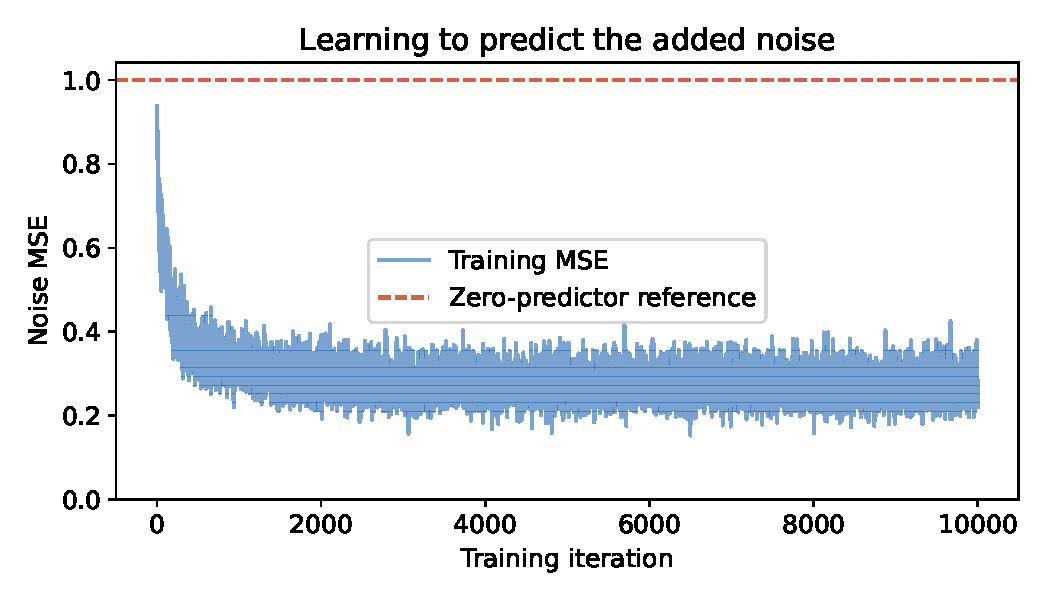
\includegraphics[width=.79\textwidth,height=.62\textheight,keepaspectratio]{figures/loss_curve.pdf}
\end{center}
\small
Always predicting zero gives expected MSE 1 per coordinate.\\[2mm]
The best predictor averages possible noises given $(x_t,t)$, so zero loss is not generally attainable.
\end{frame}

\begin{frame}{Noise prediction gives a clean-data estimate}
From $x_t=\sqrt{\bar\alpha_t}\,x_0+\sqrt{1-\bar\alpha_t}\,\varepsilon$,
\large
\[\widehat x_0=\frac{x_t-\sqrt{1-\bar\alpha_t}\,\varepsilon_\theta(x_t,t)}{\sqrt{\bar\alpha_t}}\]
\normalsize
\vspace{5mm}
This explains why predicting noise helps denoising.\\[4mm]
At high noise, the denominator is small and a one-shot estimate can be inaccurate.\\[4mm]
DDPM instead constructs a sequence of reverse transitions.
\end{frame}

\begin{frame}{6. The learned reverse mean}
\large
\[\boxed{\mu_\theta(x_t,t)=\frac{1}{\sqrt{\alpha_t}}
\left(x_t-\frac{\beta_t}{\sqrt{1-\bar\alpha_t}}\varepsilon_\theta(x_t,t)\right)}\]
\normalsize
\vspace{5mm}
The network predicts noise; the schedule converts that prediction into a mean for $x_{t-1}$.\\[4mm]
This is not simply $x_t-\varepsilon_\theta$. Both schedule factors matter.\\[4mm]
The reverse transition also needs a variance.
\ddpmref
\end{frame}

\begin{frame}[fragile]{A fixed reverse variance}
\[\tilde\beta_t=\beta_t\frac{1-\bar\alpha_{t-1}}{1-\bar\alpha_t},\qquad\bar\alpha_0=1\]
\begin{lstlisting}[basicstyle=\ttfamily\footnotesize]
alpha_bar_previous = torch.cat([torch.ones(1), alpha_bar[:-1]])
reverse_variance = beta * (1 - alpha_bar_previous) / (1 - alpha_bar)
\end{lstlisting}
\small
This is the forward posterior variance when both $x_t$ and clean $x_0$ are known.\\[3mm]
We use it as a fixed variance for the learned Gaussian reverse transition. That transition still approximates the true reverse conditional.\\[3mm]
$\tilde\beta_1=0$. The final sampling step adds no noise.
\ddpmref
\end{frame}

\begin{frame}[fragile]{Sampling: compute each reverse mean}
\begin{lstlisting}[basicstyle=\ttfamily\footnotesize]
def generate(z, stochastic=True):
    x = z.clone()
    path = [x.clone()]
    with torch.no_grad():
        for k in reversed(range(T)):
            t = torch.full((len(x), 1), (k + 1) / T)
            predicted_noise = model(torch.cat([x, t], dim=1))
            x = (x - beta[k] * predicted_noise
                 / (1 - alpha_bar[k]).sqrt()) / alpha[k].sqrt()
\end{lstlisting}
\vspace{3mm}
Python indices descend from 999 to 0. The corresponding mathematical timesteps descend from 1,000 to 1.
\end{frame}

\begin{frame}[fragile]{Sampling: add noise except at the last step}
Continuation of the same function:
\begin{lstlisting}[basicstyle=\ttfamily\footnotesize]
            if k > 0 and stochastic:
                x = x + reverse_variance[k].sqrt() * torch.randn_like(x)
            path.append(x.clone())
    return x, torch.stack(path)
\end{lstlisting}
\[x_{t-1}=\mu_\theta(x_t,t)+\sqrt{\tilde\beta_t}\,z_t\qquad(t>1)\]
\vspace{3mm}
Fresh $z_t\sim\mathcal N(0,I_2)$ at each reverse step.\\[3mm]
The default is stochastic DDPM. We use \texttt{False} only for an ablation.\\[3mm]
We do not clip coordinates to image bounds such as $[-1,1]$.
\end{frame}

\begin{frame}[fragile]{7. New Gaussian inputs generate new samples}
\begin{lstlisting}
torch.manual_seed(2026)
model.eval()
z = torch.randn(5000, 2)
real_test = sample_data(5000)
generated, path = generate(z)
\end{lstlisting}
\vspace{4mm}
\texttt{real\_test} is only for evaluation. It does not enter the sampler.\\[3mm]
\texttt{path[0]} is $x_T$; \texttt{path[T]} is the generated $x_0$.\\[3mm]
The same initial point can yield different outputs with new reverse noises.
\end{frame}

\begin{frame}{Reverse diffusion forms the four clusters}
\begin{center}
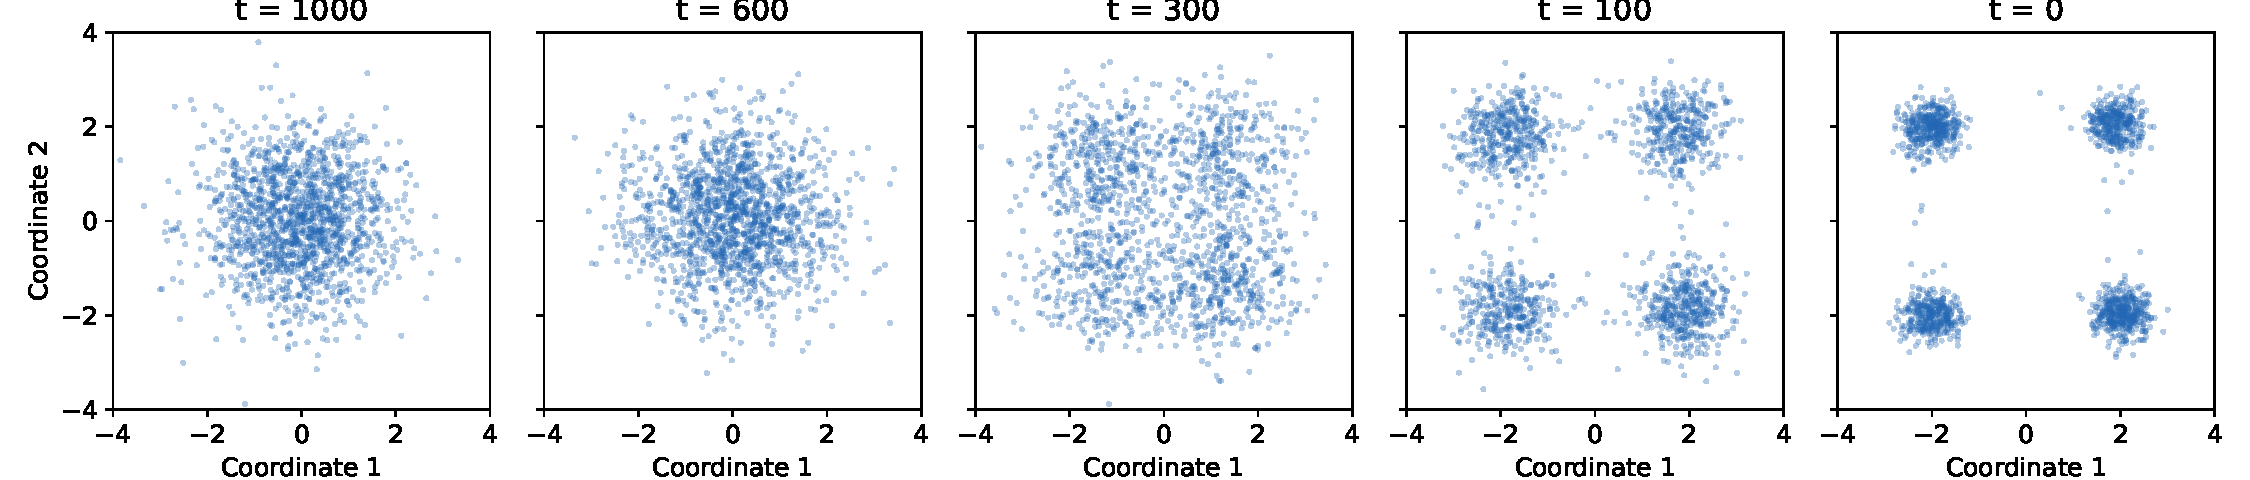
\includegraphics[width=\textwidth]{figures/reverse_sampling.pdf}
\end{center}
\vspace{5mm}
These panels follow the same 1,500 particles. Time now runs backward.\\[3mm]
Individual steps include noise even while the whole distribution develops structure.
\end{frame}

\begin{frame}{Stochastic reverse trajectories}
\begin{columns}[c]
\begin{column}{.58\textwidth}
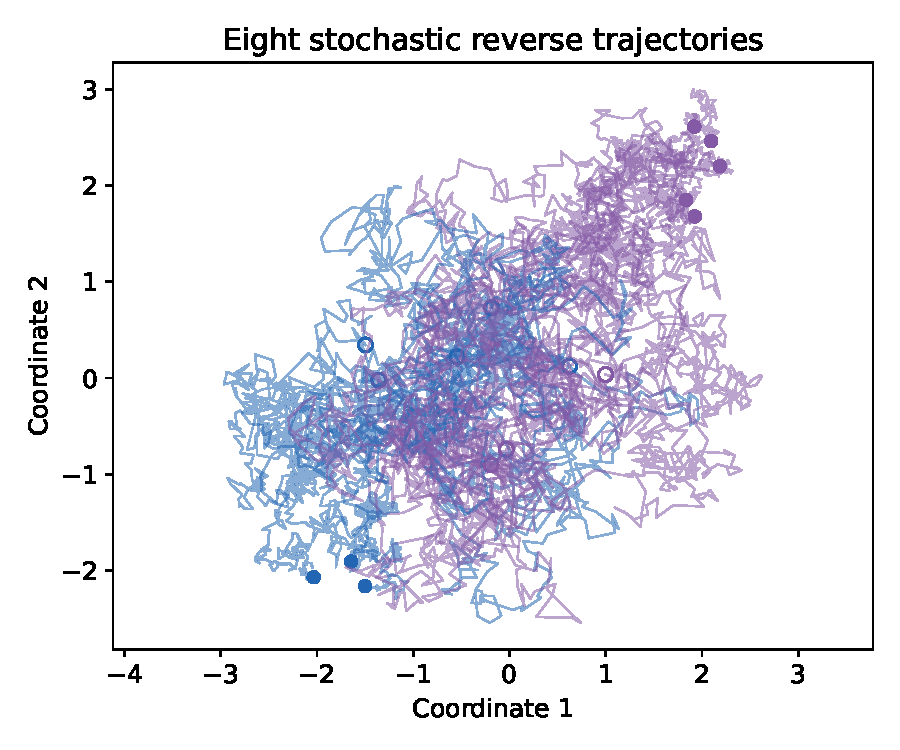
\includegraphics[width=\linewidth,height=.70\textheight,keepaspectratio]{figures/trajectories.pdf}
\end{column}
\begin{column}{.38\textwidth}
\small
Eight actual reverse paths.\\[4mm]
Open circles: initial noise.\\[4mm]
Filled dots: generated endpoints.\\[4mm]
Fresh reverse noise makes the trajectories irregular.\\[4mm]
These are sampling paths, not time series from the target data.
\end{column}
\end{columns}
\end{frame}

\begin{frame}{Generated samples compared with fresh real data}
\begin{center}
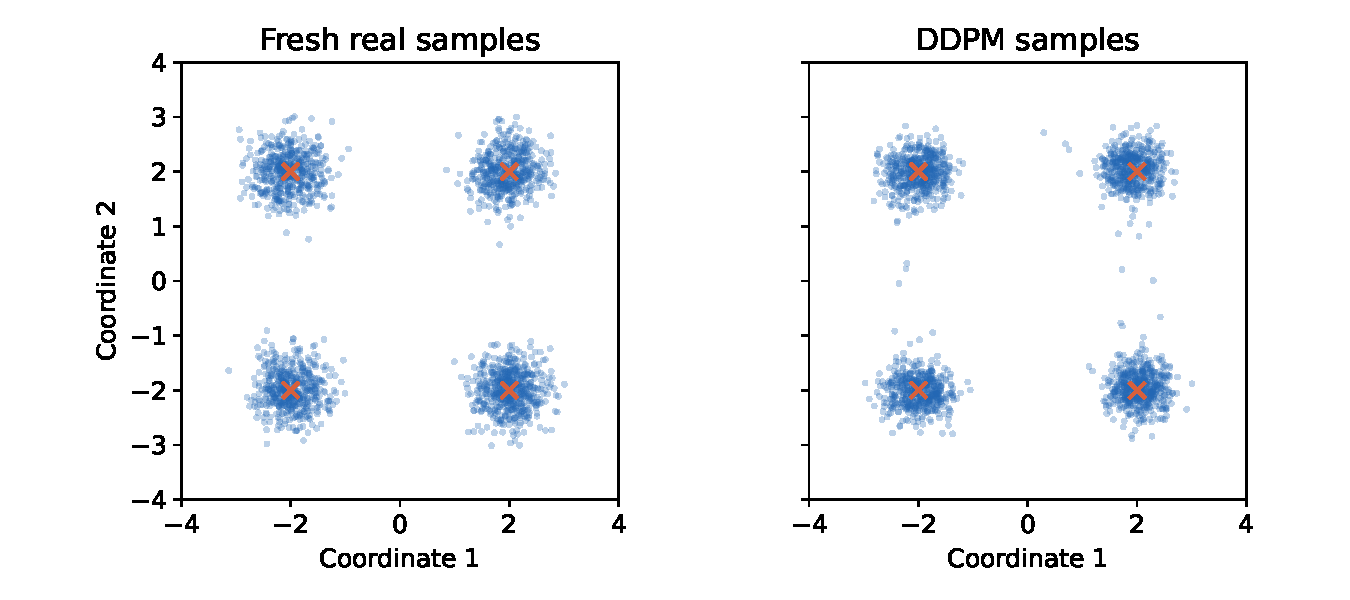
\includegraphics[width=.94\textwidth,height=.66\textheight,keepaspectratio]{figures/sample_comparison.pdf}
\end{center}
\small
Equal axes; 2,000 points shown per panel.\\[2mm]
Look for all four clusters, appropriate proportions, and the correct spread.
\end{frame}

\begin{frame}{Distribution checks on 5,000 samples}
\begin{center}
\small\begin{tabular}{lrr}
\toprule
Diagnostic & Fresh real & DDPM\\
\midrule
Nearest $(-2,-2)$ (\%) & 24.9000 & 24.7600\\[1mm]
Nearest $(-2,2)$ (\%) & 24.3800 & 26.6800\\[1mm]
Nearest $(2,-2)$ (\%) & 25.8600 & 24.1000\\[1mm]
Nearest $(2,2)$ (\%) & 24.8600 & 24.4600\\[1mm]
RMS distance to nearest center & 0.4934 & 0.4246\\[1mm]
Within distance 1 of a center (\%) & 98.4400 & 99.1400\\[1mm]
\bottomrule
\end{tabular}

\end{center}
\vspace{3mm}
Nearest-center counts check coverage; they do not identify true component labels.\\[3mm]
Smaller radius is not automatically better. A collapsed cluster has radius zero.\\[2mm]
\small These diagnostics do not certify a full distribution match.
\end{frame}

\begin{frame}{Experiment: removing reverse-step noise}
\begin{center}
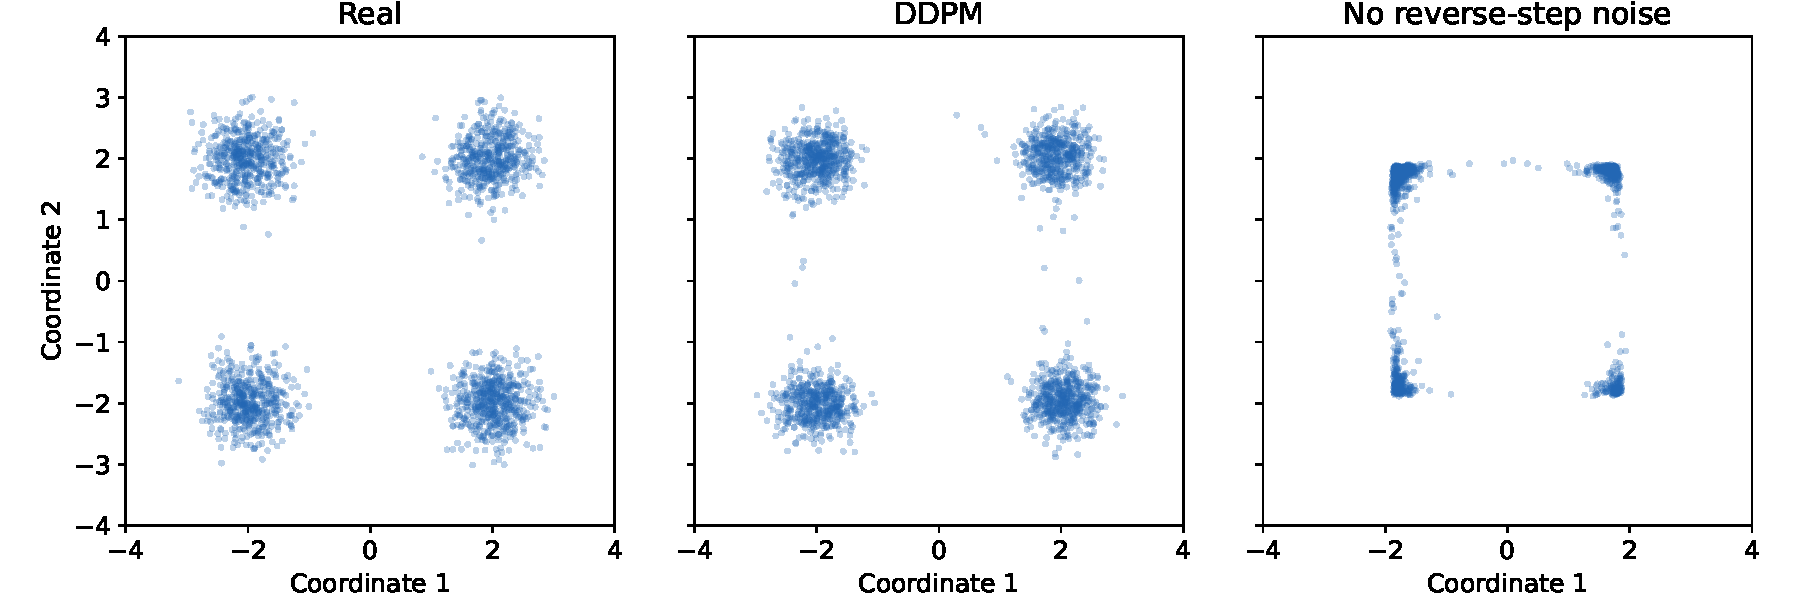
\includegraphics[width=\textwidth,height=.55\textheight,keepaspectratio]{figures/noise_ablation.pdf}
\end{center}
\small
RMS radius: real 0.4934, DDPM 0.4246, mean-only 0.4292.
\\[2mm]
Same initial noise; the mean-only clusters shift inward and change shape.\\[2mm]
Similar RMS radii do not imply similar distributions.\\[2mm]
This mean-only chain is not DDIM or a probability-flow ODE.
\end{frame}

\begin{frame}{Experiments and further reading}
\begin{enumerate}\setlength\itemsep{3mm}
\item Change the seed or reduce training to 2,000 iterations.
\item Make the target clusters narrower and examine their learned widths.
\item Shorten $T$ and check $\bar\alpha_T$ before retraining.
\item Keep the same starting point and change the reverse noise draws.
\end{enumerate}
\vspace{3mm}
Do not simply skip timesteps with the original one-step coefficients.\\[2mm]
Use fresh test data after tuning. These examples are not a controlled ranking of DDPM versus ODE generation.
\vfill
\tiny References: \href{https://arxiv.org/abs/2006.11239}{Ho et al. (2020), DDPM};
\href{https://github.com/hojonathanho/diffusion}{authors' implementation};
\href{https://arxiv.org/abs/2010.02502}{Song et al., DDIM}.\\[2mm]
\small Companion notebook: \texttt{learning\_ddpm.ipynb}
\end{frame}

\end{document}
